\section{Sp\-Random.h File Reference}
\label{SpRandom_8h}\index{SpRandom.h@{SpRandom.h}}


This graph shows which files directly or indirectly include this file:\begin{figure}[H]
\begin{center}
\leavevmode
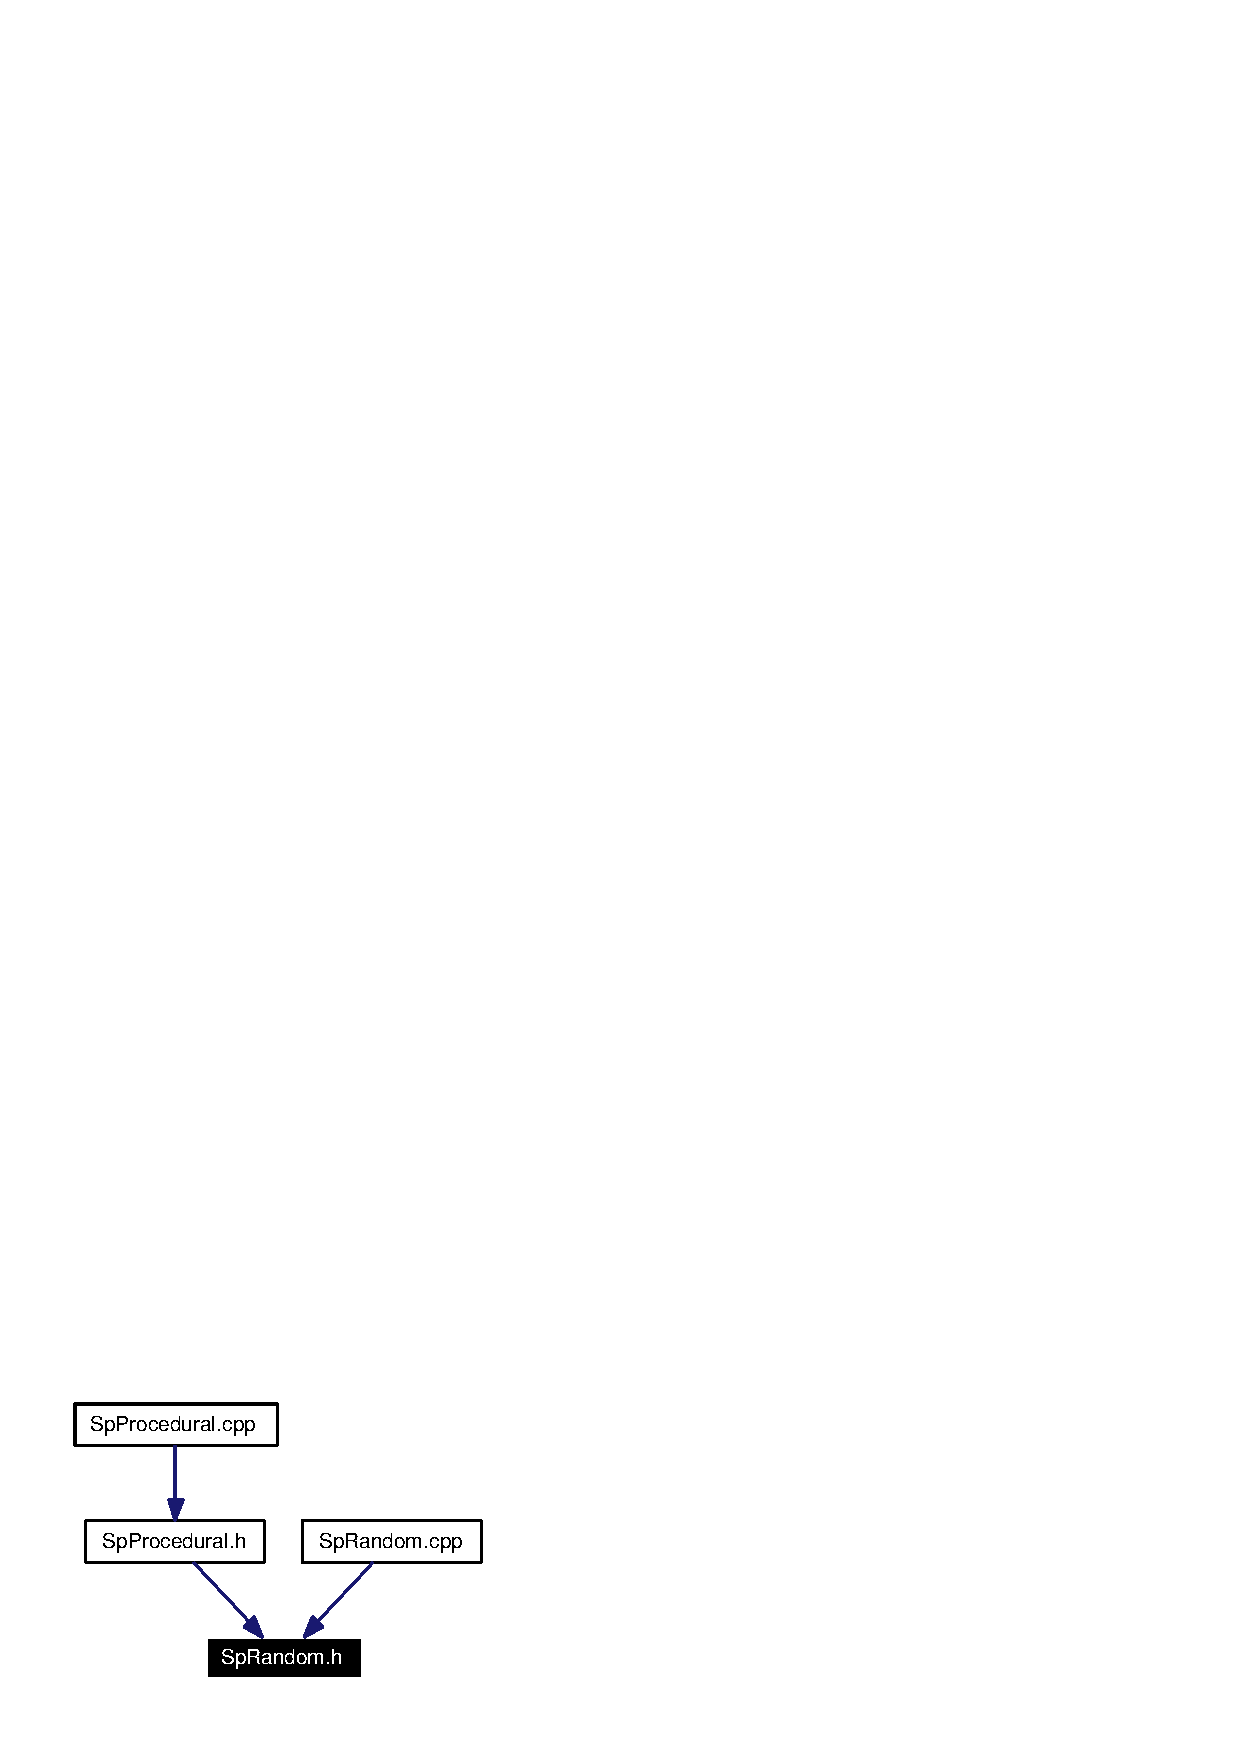
\includegraphics[width=116pt]{SpRandom_8h__dep__incl}
\end{center}
\end{figure}
\subsection*{Namespaces}
\begin{CompactItemize}
\item 
namespace {\bf Spark}
\end{CompactItemize}
\subsection*{Functions}
\begin{CompactItemize}
\item 
void {\bf Seed\-Random} (unsigned long seed)
\begin{CompactList}\small\item\em Initializes the random number table. \item\end{CompactList}\item 
unsigned int {\bf Random\-UInt} (void)
\begin{CompactList}\small\item\em Generates a random 32bit unsigned int. \item\end{CompactList}\item 
float {\bf Random\-Unit\-Float} (void)
\begin{CompactList}\small\item\em Generates a random real number on [0,1]-real-interval. \item\end{CompactList}\item 
float {\bf Random\-Unit\-Open\-Float} (void)
\begin{CompactList}\small\item\em Generates a random real number on [0,1)-real-interval. \item\end{CompactList}\item 
float {\bf Random\-Symmetric\-Float} (void)
\begin{CompactList}\small\item\em Generates a random real number on [-1,1]. \item\end{CompactList}\item 
float {\bf Random\-Interval\-Float} (float f\-Min, float f\-Max)
\begin{CompactList}\small\item\em Generates a random real number on [-min, max]. \item\end{CompactList}\end{CompactItemize}


\subsection{Function Documentation}
\index{SpRandom.h@{Sp\-Random.h}!RandomIntervalFloat@{RandomIntervalFloat}}
\index{RandomIntervalFloat@{RandomIntervalFloat}!SpRandom.h@{Sp\-Random.h}}
\subsubsection{\setlength{\rightskip}{0pt plus 5cm}float Random\-Interval\-Float (float {\em f\-Min}, float {\em f\-Max})\hspace{0.3cm}{\tt  [inline]}}\label{namespaceSpark_a117}


Generates a random real number on [-min, max]. 

Definition at line 88 of file Sp\-Random.h.

References Spark::Random\-Unit\-Float().\index{SpRandom.h@{Sp\-Random.h}!RandomSymmetricFloat@{RandomSymmetricFloat}}
\index{RandomSymmetricFloat@{RandomSymmetricFloat}!SpRandom.h@{Sp\-Random.h}}
\subsubsection{\setlength{\rightskip}{0pt plus 5cm}float Random\-Symmetric\-Float (void)\hspace{0.3cm}{\tt  [inline]}}\label{namespaceSpark_a116}


Generates a random real number on [-1,1]. 

Definition at line 80 of file Sp\-Random.h.

References Spark::Random\-Unit\-Float().

Referenced by Spark::Sp\-Vertex\-Noise\-Sb::initialize().\index{SpRandom.h@{Sp\-Random.h}!RandomUInt@{RandomUInt}}
\index{RandomUInt@{RandomUInt}!SpRandom.h@{Sp\-Random.h}}
\subsubsection{\setlength{\rightskip}{0pt plus 5cm}unsigned int Spark::Random\-UInt (void)}\label{namespaceSpark_a113}


Generates a random 32bit unsigned int. 

Definition at line 70 of file Sp\-Random.cpp.

References LOWER\_\-MASK, M, MATRIX\_\-A, N, Spark::Seed\-Random(), and UPPER\_\-MASK.

Referenced by Spark::Sp\-Vertex\-Noise\-Sb::initialize(), Spark::Random\-Unit\-Float(), and Spark::Random\-Unit\-Open\-Float().\index{SpRandom.h@{Sp\-Random.h}!RandomUnitFloat@{RandomUnitFloat}}
\index{RandomUnitFloat@{RandomUnitFloat}!SpRandom.h@{Sp\-Random.h}}
\subsubsection{\setlength{\rightskip}{0pt plus 5cm}float Spark::Random\-Unit\-Float (void)}\label{namespaceSpark_a114}


Generates a random real number on [0,1]-real-interval. 

Definition at line 112 of file Sp\-Random.cpp.

References Spark::Random\-UInt().

Referenced by Spark::Random\-Interval\-Float(), and Spark::Random\-Symmetric\-Float().\index{SpRandom.h@{Sp\-Random.h}!RandomUnitOpenFloat@{RandomUnitOpenFloat}}
\index{RandomUnitOpenFloat@{RandomUnitOpenFloat}!SpRandom.h@{Sp\-Random.h}}
\subsubsection{\setlength{\rightskip}{0pt plus 5cm}float Spark::Random\-Unit\-Open\-Float (void)}\label{namespaceSpark_a115}


Generates a random real number on [0,1)-real-interval. 

Definition at line 119 of file Sp\-Random.cpp.

References Spark::Random\-UInt().\index{SpRandom.h@{Sp\-Random.h}!SeedRandom@{SeedRandom}}
\index{SeedRandom@{SeedRandom}!SpRandom.h@{Sp\-Random.h}}
\subsubsection{\setlength{\rightskip}{0pt plus 5cm}void Spark::Seed\-Random (unsigned long {\em seed})}\label{namespaceSpark_a112}


Initializes the random number table. 

Definition at line 51 of file Sp\-Random.cpp.

References N.

Referenced by Spark::Sp\-Vertex\-Noise\-Sb::initialize(), and Spark::Random\-UInt().